\section{Conclusiones}
\label{sec:conclusiones}

\subsection{Evaluación del proyecto}

La evaluación del proyecto en general es muy positiva, habiéndose cumplido tanto con todos los objetivos iniciales como con los requisitos definidos.

Todo el proyecto ha sido desarrollado en la plataforma \textit{Google Colab}, la cual presenta una serie de limitaciones en cuando a la capacidad del hardware disponible y en cuanto al tiempo de uso del mismo. Las limitaciones de capacidad del hardware han impactado al entrenamiento, teniendo que limitar tanto el tamaño de la red como el \textit{batch size} de la red. Las limitaciones de tiempo de uso han forzado realizar el entrenamiento de los modelos en varias fases, sobre todo los más grandes. En cada fase se ha realizado una transferencia de conocimiento, teniendo como punto de partida el modelo resultante de la fase anterior, salvo en la fase inicial, que se tiene como punto de partida el modelo entrenado publicado por los autores de YOLO. Tras finalizar cada fase se ha realizado una evaluación del modelo obtenido y se ha comparado con el de la fase anterior para decidir si se prosigue con el entrenamiento.

Los modelos han sido entrenados pocas épocas debido a la gran cantidad de tiempo que requería el entrenamiento y por la limitación de tiempo de uso del hardware. Hoy en día, la plataforma Google Colab no está pensada para hacer un uso muy intensivo de la misma. Si es el caso y se lleva la infraestructura a sus límites, eres penalizado y las sucesivas solicitudes de hardware son rechazadas. Para el entrenamiento de varios de los modelos se ha llevado la plataforma al límite en repetidas ocasiones, haciendo uso de toda la capacidad de GPU (12 GB) y de todo el tiempo de uso disponible (12 horas). Así como en la fase inicial de entrenamiento era sencillo conseguir la asignación de recursos, en la fase final ha ocurrido lo contrario, resultando difícil la asignación de recursos, teniendo que solicitarlos repetidas ocasiones durante varias horas hasta conseguirlos finalmente.

Al transformar los modelos a TFLite y evaluarlos desde python y java y contrastar los resultados, estos no son exactamente iguales. Existen pequeñas diferencias en las salidas del modelo a partir del 4-6 decimal. No se ha encontrado una explicación para esto, aunque estas diferencias no alteran demasiado las predicciones.

El tiempo de la inferencia en el dispositivo móvil ha resultado superior al esperado, obteniendo unos valores bajos de \textit{FPS} para las imágenes procesadas. Con un móvil de gama media (Nokia 7 plus) se alcanzan los 5-7 FPS. Con un móvil de gama alta (OnePlus 7 pro) se alcanzan unos 12 FPS.

\subsection{Posibles mejoras y trabajos futuros}

El principal punto de mejora se encuentra en los datos utilizados para el proyecto y se ven dos vías de mejora: una relacionada con el tamaño del conjunto de datos y otra relacionada con el etiquetado del mismo.

La primera de las líneas de mejora, y que es sencilla de aplicar, está relacionada con el volumen de datos. Se trata de cambiar el balance entre las imágenes de entrenamiento y las de test (actualmente 70-30). Utilizándose el mismo juego de datos, podría hacerse otra organización de los subconjuntos para obtener un balance 80-20. Consiguiendo así un mayor número de imágenes de entrenamiento.

Con respecto al etiquetado de los datos, se ha observado que existen imágenes en las cuales hay baches que no han sido etiquetados y baches etiquetados con regiones que no se ajustan demasiado bien al bache. Para los algoritmos de detección de objetos es importante etiquetar todos los objetos existentes en la imagen y que las regiones se ajusten lo máximo posible al objeto real. Otra de las líneas de mejora, más costosa que la anterior, consiste en una revisión del etiquetado de las imágenes.

Tras ver las diferencias de los resultados obtenidos con las imágenes originales y con las imágenes propias, se han analizado las características de los baches de ambos conjuntos y se han observado notables diferencias. En las imágenes originales, los baches presentan priedras, arena y hojas. Sin embargo, en las imágenes propias, debajo de los baches hay más asfalto, debido a que las carreteras son reasfaltadas y los baches dejan al descubierto el asfalto original (ejemplo en figura \ref{fig:pothole_diffs}). Otra vía de mejora, también costosa, sería la incorporación de imágenes de baches obtenidas en España al conjunto de datos existente.

\begin{figure}[H]
	\centering
	\begin{subfigure}[h]{0.45\linewidth}
		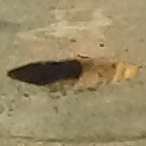
\includegraphics[width=\linewidth]{images/pothole_diff_orig.png}
	\end{subfigure}
	\begin{subfigure}[h]{0.45\linewidth}
		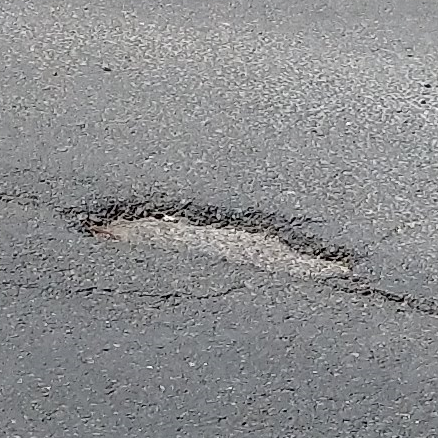
\includegraphics[width=\linewidth]{images/pothole_diff_esp.png}
	\end{subfigure}
	\caption{A la izquierda un ejemplo de bache típico presente en las imágenes originales. A la derecha un ejemplo de bache típico de las imágenes de España}
	\label{fig:pothole_diffs}
\end{figure}

Uno de los factores más determinantes para la precisión obtenida por los modelos ha sido el tamaño de los baches con respecto al de la imagen. Otra vía de mejora, también muy costosa, consistiría en crear un nuevo juego de datos en el que las fotos hayan sido tomadas desde el exterior del vehículo y con un encuadre de tal forma que los baches, aun siendo pequeños, tengan un tamaño representativo en la imagen. Esto podría conseguirse encuadrando la zona del asfalto frente al vehículo sin que aparezca paisaje al fondo ni en los laterales.

El rendimiento del modelo en el dispositivo móvil es otro de los aspecto a mejorar. Existen otro tipo de transformaciones que se pueden hacer sobre el modelo para obtener uno \textit{quantized} \cite{s8_quantizedmodel}, pudiendo llegar a incrementar su rendimiento x3.

El soporte de la GPU en \textit{TFLite} se encuentra actualmente en fase experimental. Hoy en día es bastante frecuente que los dispositivos móviles tengan incorporada una GPU, por lo que sería muy interesante poder hacer uso de la misma. En la aplicación móvil se ha hecho uso de la misma, aunque no se ha obtenido una mejora, debido precisamente a que se encuentra en fase experimental y a que una de las operaciones del modelo (\textit{BatchNormalization}) \cite{s8_batchnormalization} no se encuentra soportada por el momento. Bien podría esperarse a que se soporte esta operación o bien se podría estudiar hacer una variación del modelo para remplazar esta operación por otra soportada sin que se afecte a la precisión del mismo.

\subsection{Conclusiones personales}

El proyecto me ha resultado un reto desafiante y gratificante ya que me ha permitido ampliar mis conocimientos haciendo un simulacro de lo que podría ser un proyecto profesional.

Tener un juego de datos con abundantes imágenes y correctamente etiquetadas es clave para obtener buenos resultados. Pero esto no es suficiente, ya que al igual que ocurre con otras técnicas es primordial conocer los datos. Gracias al estudio del aspecto y tamaño de los baches he podido adaptar el tratamiento inicial de las imágenes y también crear distintos subconjuntos de entrenamiento que han mejorado los resultados del modelo.

Si la detección de objetos es un problema complejo a resolver, creo que la detección de objetos pequeños incrementa bastante la complejidad en todos los aspectos: etiquetado de imágenes, entrenamiento y evaluación del modelo.

Aunque el número de \textit{FPS} alcanzados en el dispositivo móvil es inferior al esperado, he conseguido alcanzar una cifra que permite una fluidez aceptable. Como se ha comentado en el punto anterior, existen múltiples vías de mejora de este apartado que creo que conseguirían mejorar este aspecto y hacer el producto válido para un uso productivo.